

\section{Related Work}
\label{sec:relate}

Recent advances in quantization \cite{dettmers2022gpt3int8, frantar2022gptq, lin2023awq, li2024svdquant, van2025fptquant, tao2025plug, li2025mbq, li2024evaluating, zhao2025viditq, shang2023post, li2023q, zhao2024mixdq, lin2024duquant, huang2025qvgen,tang2024post,liu2024eda,sui2024bitsfusion} have significantly improved model efficiency. For matrix multiplication $\mathbf{Y} = \mathbf{X}\mathbf{W}^\top$, where $\mathbf{X} \in \mathbb{R}^{k \times n}$ and $\mathbf{W} \in \mathbb{R}^{m \times n}$, common strategies for maintaining high accuracy include:


\paragraph{1) Per-channel Scaling.} This method\cite{xiao2022smoothquant} mitigates outliers by applying a diagonal scaling matrix $\text{diag}(\mathbf{c})$ to transfer outlier energy from $\mathbf{X}$ to $\mathbf{W}$: $\mathbf{Y} = (\mathbf{X} \text{diag}(\mathbf{c})^{-1}) \cdot (\text{diag}(\mathbf{c})\mathbf{W}^\top)$.

\paragraph{2) Rotation Transformation.} A more general approach uses a transformation matrix $\mathbf{H}$ and its inverse transpose $\mathbf{H}^{-\top}$ such that $\mathbf{Y} = (\mathbf{X}\mathbf{H})(\mathbf{W}\mathbf{H}^{-\top})^\top$. Orthogonal rotations (e.g., Hadamard)\cite{ashkboos2024quarot} redistribute outlier energy across channels to reduce maximum values within each matrix (\textit{intra-matrix}). Non-orthogonal invertible transforms act as a composite of rotation and scaling.

\paragraph{\textbf{Low-bit Attention in Video Generation.}} Current low-bit video attention methods focus on quantizing $\mathbf{Q}\mathbf{K}^\top$ and $\mathbf{P}\mathbf{V}$ using alternative techniques:
(1) \textbf{QKV Smoothing:} The SageAttention series \cite{zhang2025sageattention1, zhang2025sageattention2} uses INT4/INT8 formats, employing channel smoothing (e.g., $\mathbf{Q} - \mathbb{E}[\mathbf{Q}]$) to suppress biased outliers. SageAttention3~\cite{zhang2025sageattention3} further extends this line with NVFP4 micro-scaling formats.
(2) \textbf{Token Reordering:} PAROAttention \cite{zhao2025paroattention} reorders tokens in $\mathbf{Q}$, $\mathbf{K}$, and $\mathbf{V}$ so that each block of $\mathbf{P}$ contains values with similar magnitudes, thereby improving per-block quantization precision. This token-level strategy is \emph{complementary} to our channel-level rotation approach and can potentially be combined for further gains.



\paragraph{\textbf{Low-bit Attention in LLMs.}} LLM quantization typically targets the memory-bound KV cache \cite{liu2026pmkvq}. To mitigate quantization error, rotation-based methods like FlatQuant and SpinQuant\cite{sun2025flatquant,liu2025spinquant} utilize invertible transforms, while \textbf{QuaRot} \cite{ashkboos2024quarot} employs Hadamard matrices. Recent advances, such as FlashAttention-3 \cite{shah2024flashattention}, further optimize efficiency by reducing rotation overhead within high-performance kernels.



\paragraph{\textbf{Key Differences: LLM vs. 3D-RoPE Video DiTs.}}
Fig.~\ref{fig:llmvsd} illustrates the key differences between LLM decoding and 3D-RoPE video DiT attention, highlighting why rotation strategies designed for LLM KV-cache quantization do not directly transfer to DiT-based video generation models with 3D RoPE.

We identify two fundamental distinctions:
(1) \textbf{Computational Intensity:} LLM decoding is memory-bound~\cite{patel2024splitwise,qin2024mooncake,zhong2024distserve}, allowing online rotations to overlap with RoPE or attention kernels. In contrast, 3D-RoPE video DiTs are compute-bound, making online rotation overhead significant and difficult to hide.
(2) \textbf{Quantization Symmetry:} LLM quantization often keeps $\mathbf{Q}$ in FP16 and only quantizes $\mathbf{K}$ for the KV-cache. Conversely, 3D-RoPE video DiTs require simultaneous quantization of $\mathbf{Q}$ and $\mathbf{K}$ to leverage low-bit matmul hardware for actual speedup.



\begin{figure*}[t]
    \centering
    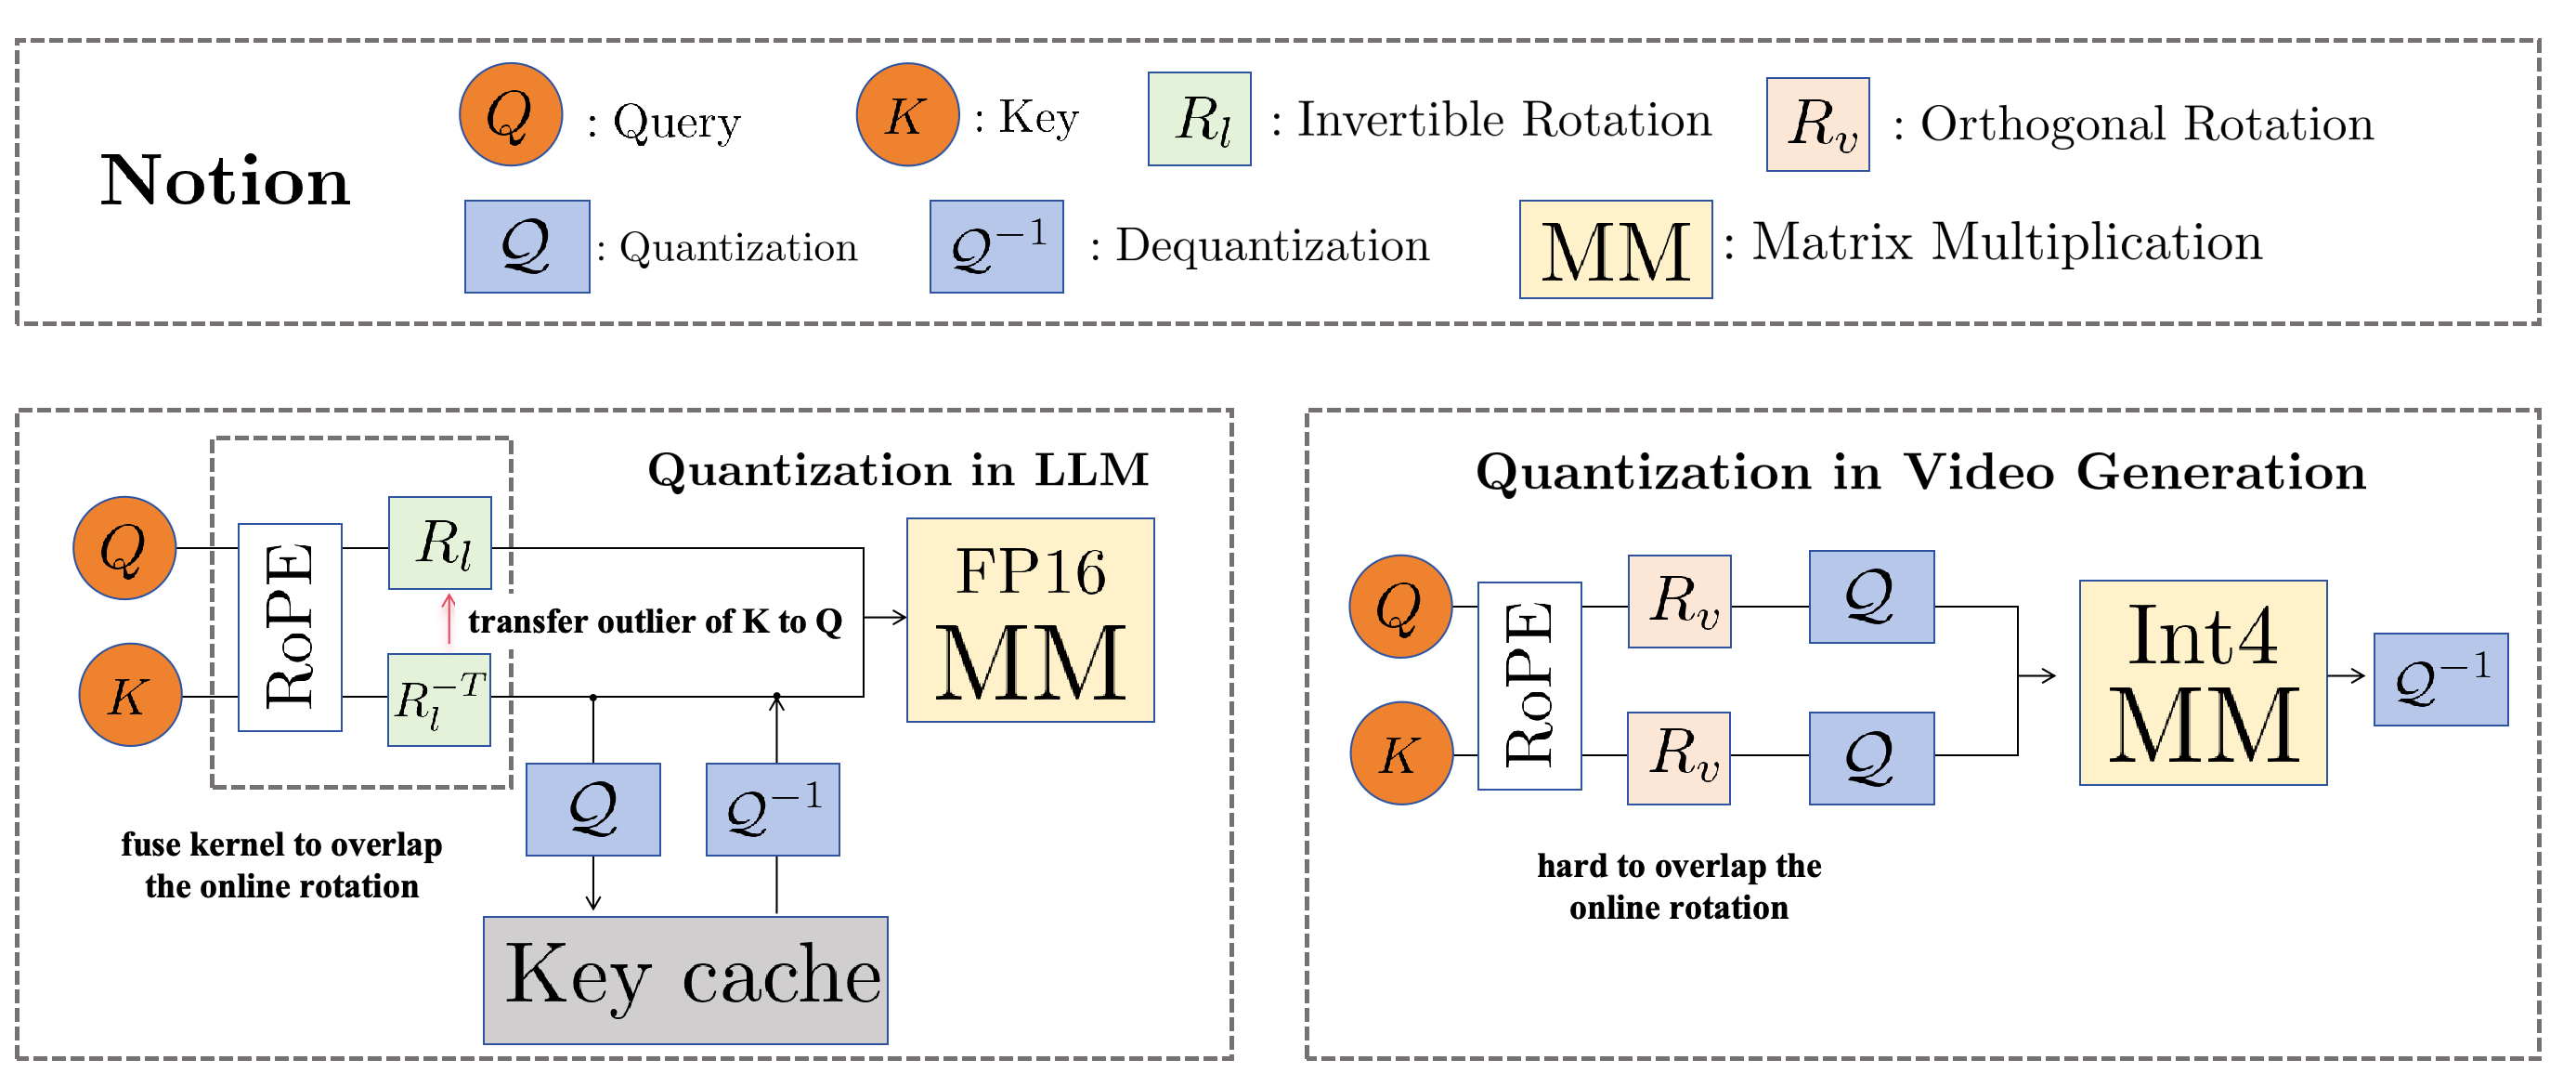
\includegraphics[width=1\linewidth]{eccv2026/samll_2/llmvsd.png}
    \caption{\textbf{Quantization differences between LLM decoding and 3D-RoPE video DiTs}. In LLMs, rotations can prioritize $\mathbf{K}$ quantization and transfer part of the outlier burden to $\mathbf{Q}$. In 3D-RoPE video DiTs, both $\mathbf{Q}$ and $\mathbf{K}$ must be quantized simultaneously, which requires orthogonal transforms and low-overhead execution.}
    \label{fig:llmvsd}
\end{figure*}

Furthermore, we extend Hadamard transforms to the Value ($\mathbf{V}$) matrix. While previously used in LLM KV-caches, we formally prove their compatibility with smoothing for $\mathbf{V}$. By bridging these rotation strategies and enhancing $\mathbf{P}$ quantization, \textbf{RotateAttention} significantly improves mixed-precision INT4 attention quality for 3D-RoPE video DiTs.
